\chapter{REGISTRASI DAN TRANSFORMASI KOORDINAT}

\begin{enumerate}[1.]
  \item Pilih File -\textgreater Open
  
  \item Cari file \textbf{peta} yang berbentuk gambar, seperti misalnya gambar dengan format \textbf{tif}, caranya, pilih \textbf{Files of Types} -\textgreater \textbf{Raster Image} seperti tampilan jendela berikut ini :
  
  \begin{figure}[H]
    \centering
    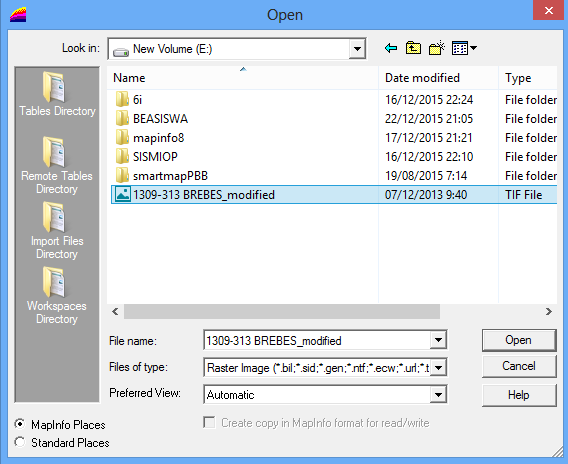
\includegraphics[width=1\textwidth]{./resources/048-membuka-file-raster}
    \caption{Jendela Untuk Membuka File Raster}.
  \end{figure}
  
  \item Buka \textit{file} \textbf{peta} tersebut sehingga muncul jendela pernyataan bahwa gambar yang akan dibuka belum terregistrasi, kemudian pilih \textbf{Register}. Jendelanya akan tampil seperti ini :
  
  \begin{figure}[H]
    \centering
    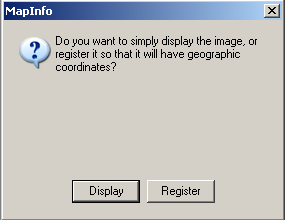
\includegraphics[width=1\textwidth]{./resources/049-a-jendela-register}
    \caption{Jendela Pernyataan Register}
  \end{figure}
  
  \item Pilih \textbf{Projection} sehingga muncul jendela \textit{image registration} seperti ini :
  
  \begin{figure}[H]
    \centering
    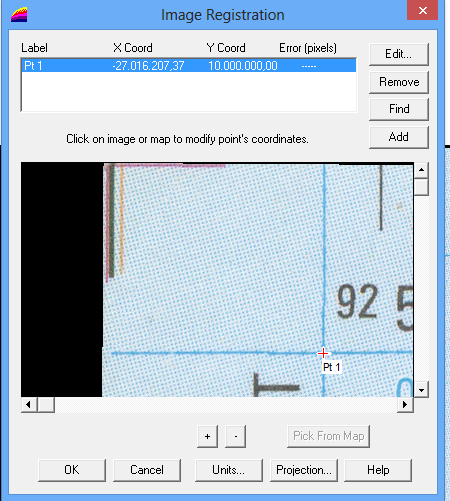
\includegraphics[width=1\textwidth]{./resources/051-jendela-image-registration}
    \caption{Jendela Image Registration}
  \end{figure}
    
  \item Masukan koordinat pertama pada titik GCP ke-satu dengan meng-klik \textbf{Add}. Lakukan hal yang sama pada titik-titik GCP berikutnya dilakukan searah jarum jam. Perhatikan Error RMS-nya. Edit Image X dan Image Y-nya sampai pada kolom Error menjadi 0. Perlu juga dilakukan perumusan dari koordinat yang ada pada data raster menjadi data UTM.
\end{enumerate}

